\nnarticleheader{A Model of Shear-Induced Fibrillogenesis}{Dr. Holly M Golecki, Professor, University of Illinois at Urbana-Champaign}
Fibrillar proteins that support cells and tissues\textit{in vivo} are part of the extracellular matrix
(ECM). One ECM protein, fibronectin (FN), may play a significant role in organization, support
and development of the skin. In development, fetal skin contains high concentrations of FN.
These high expression levels also correspond with scarless healing after dermal injury. During
aging, highly elastic FN breaks down and is replaced by stiffer collagen. When a wound occurs
in adult skin, the healed tissue forms a dense collagen-rich ECM called a scar. We asked if
fibrillar FN applied to adult wounds could “trick” the microenvironment in assuming a fetal
phenotype and promote scarless healing in adults. This task presents a challenge as currently
available manufacturing techniques for protein fiber engineering have limited production rates.

\renewcommand{\thefigure}{1}
\begin{figure}[h]
  \begin{center}
    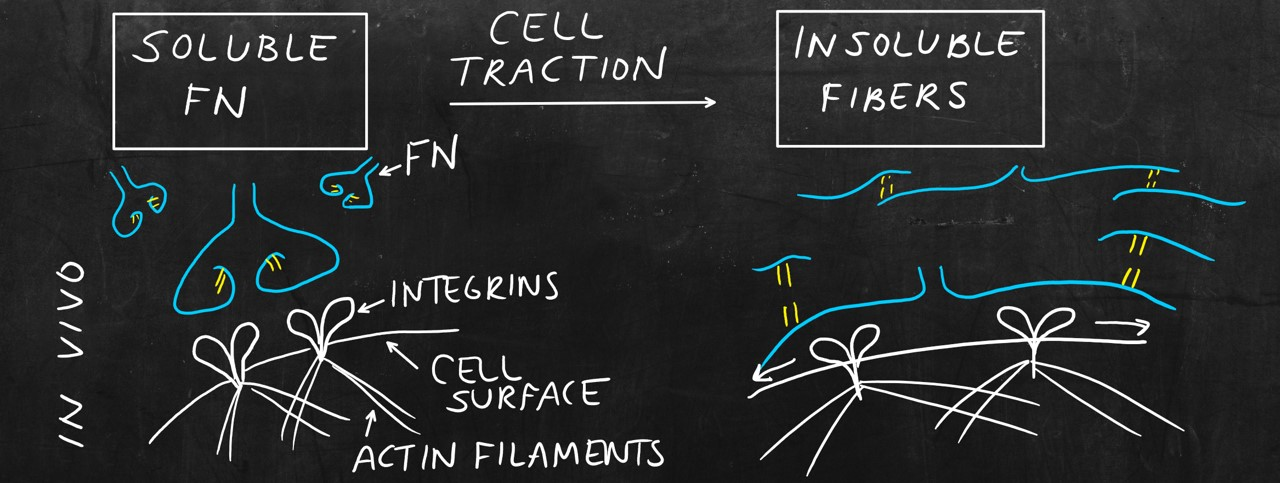
\includegraphics[width=\textwidth]{golecki_figure_1}
  \end{center}
  \caption{FN structure and unfolding in vivo. Schematic of the mechanism of FN fibrillogenesis.}
\end{figure}

To engineer fibrillar FN, we must first understand how it is built in vivo. Soluble,
globular FN circulates in the blood. Cells attach to FN via integrin binding receptors that transfer
mechanical traction forces to unfold FN. This unfolding exposes cryptic binding sites inducing
fibrillogenesis (Figure 1). The challenge is to replicate that process outside the body, turning fibrillogenesis into a manufacturing process. We propose that a perforated reservoir rotating at
high speeds may propel protein solutions out of the reservoir orifice stretching, drying and
solidifying nanofibers. Within that process we hypothesized that shear forces within the reservoir
are capable of unfolding FN inducing fibrillogenesis on the benchtop. Herein we describe a fluid
dynamics model of shear induced fibrillogenesis using this system to manufacture FN nanofibers
for future use in wound dressings.

\noindent
\textbf{Shear Fluid Model}

To test this hypothesis, we developed a mathematical model that predicts how shear forces generated using a spinning orifice can be used to induce the high-throughput production of FN nanofibers. Others have probed single FN molecules to determine tensile forces required to unfold FN. We used Mohr’s circle \cite{gere} to determine the shear stress required to unfold FN by translating values from single molecule uniaxial tensile tests \cite{oberhauser} to shear. Mohr’s circle is a graphical representation of the relationship between principle and shear stress. We calculated 3.7 kPa as the minimum shear stress required to unfold a FN molecule. Next, to calculate the shear produced by a spinning orifice, we derived a model from Navier Stokes for the shear stress distribution through the diameter of the orifice.

\renewcommand{\thefigure}{2}
\begin{figure}[h]
  \begin{center}
    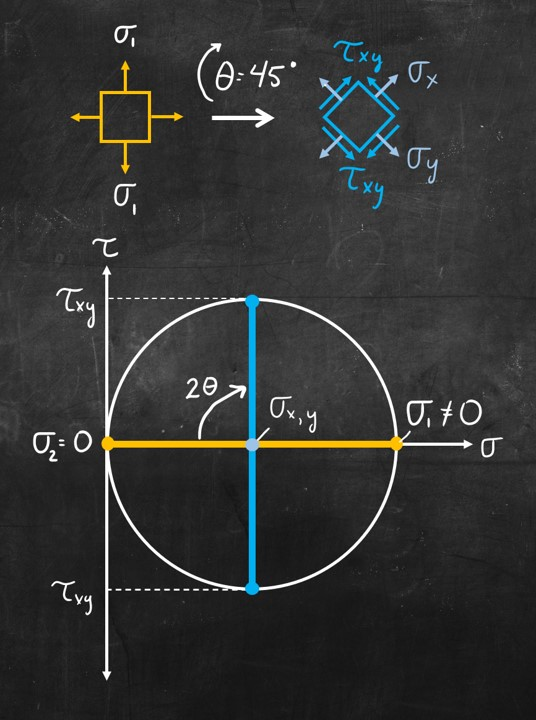
\includegraphics[scale=.55]{golecki_figure_2}
  \end{center}
  \caption{Mohr's circle for plane stress.}
\end{figure}

\renewcommand{\thefigure}{3}
\begin{figure}[h]
  \begin{center}
    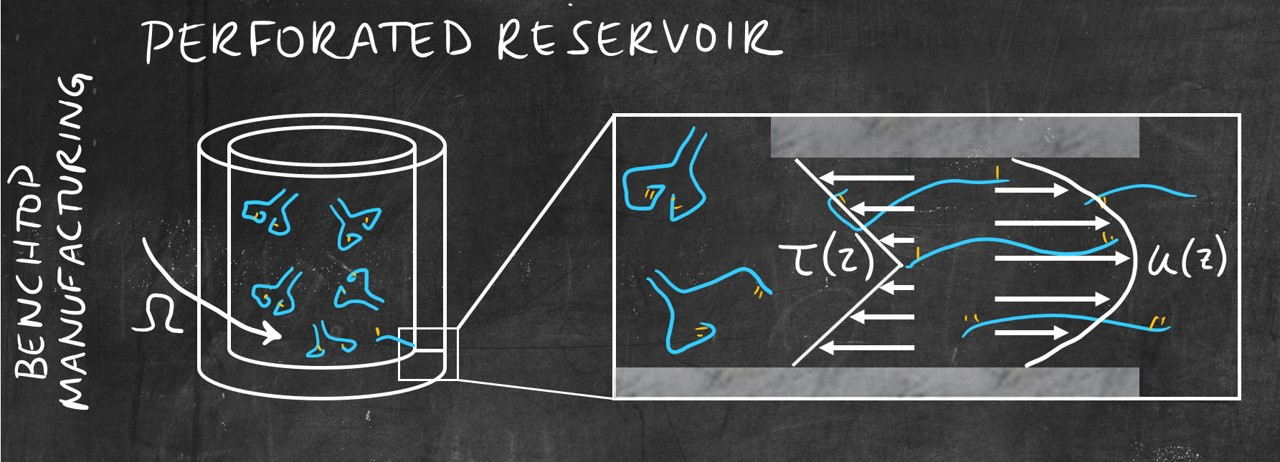
\includegraphics[scale=.5]{golecki_figure_3}
  \end{center}
  \caption{Schematic representing hypothesized benchtop shear unfolding in a rotating perforated reservoir.}
\end{figure}

\noindent
\textbf{Details of Shear Fluid Model}

To derive an equation of fluid flow through the orifice, we modeled shear stresses in a Poiseuille flow rotating with angular speed ($\Omega$). The system consists of a viscous, incompressible, fluid flowing through a tube of uniform cross section, rotating about the Y axis, applying the  following assumptions:

\begin{center}
1. The flow is steady and does not change with time: $\frac{du_z}{dt}=0$.\\
1a. Flow is in unidirectional: $u_r = 0; u_\theta = 0$.\\
2. The flow is axisymetric.
\end{center}

\renewcommand{\thefigure}{4}
\begin{figure}[h]
  \begin{center}
    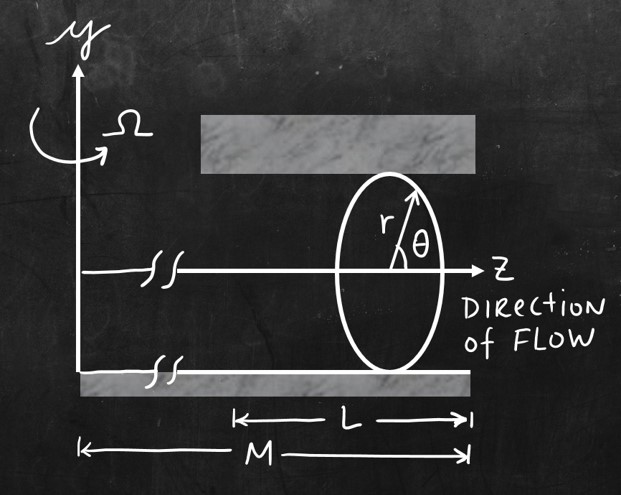
\includegraphics[scale=.42]{golecki_figure_4}
  \end{center}
  \caption{Schematic of reservoir orifice.}
\end{figure}

\noindent
\textit{Conservation of Mass (from the continuity equation):}
\[\frac{\partial}{\partial t}\rho 
+ \frac{1}{r}\frac{\partial r u_r}{\partial r}
+ \frac{1}{r}\frac{\partial r u_\theta}{\partial \theta}
+ \frac{\partial u_z}{\partial z}
= 0
\]

If density, $\rho$, does not change with time, there is no flow in the $r$ direction, then fluid speed does not change along the $z$ direction.
\[\frac{\partial u_z}{\partial z} = 0\]

\noindent
\textit{Conservation of Momentum:}

A very common case of Navier Stokes in cylindrical coordinates is axisymetric flow assuming no tangential velocity. The remaining quantities are independent of $\theta$. Therefore, N-S$_\theta$ goes to zero. Because we assume no flow in the $r$ direction, hydrostatic pressure is negligible, and $\frac{\partial u_z}{\partial z} = 0$ from continuity equation, N-S$_r$ goes to zero as well. From here, we study N-S in the $z$-direction:


\noindent
\textbf{References}
\begingroup
\renewcommand{\section}[2]{}% https://tex.stackexchange.com/questions/22645/hiding-the-title-of-the-bibliography
%\renewcommand{\chapter}[2]{}% for other classes
\begin{thebibliography}{3}
\bibitem{gere}
Gere, J. M. (2003). Mechanics of Materials: Thompson-Engineering.

\bibitem{oberhauser}
Oberhauser, A. F., Badilla-Fernandez, C., Carrion-Vazquez, M., and Fernandez, J. M. (2002).
The mechanical hierarchies of fibronectin observed with single-molecule AFM. 
\textit{Journal of Molecular Biology}, 319(2), 433-447. doi:10.1016/s0022-2836(02)00306-6

\bibitem{sawicka}
Sawicka, K. M., Seeliger, M., Musaev, T., Macri, L. K., and Clark, R. A. (2015). Fibronectin
interaction and enhancement of growth factors: importance for wound healing. 
\textit{Advances in wound care}, 4(8), 469-478.

\end{thebibliography}